% !TEX TS-program = pdflatex
% !TEX encoding = UTF-8 Unicode

% This is a simple template for a LaTeX document using the "article" class.
% See "book", "report", "letter" for other types of document.

\documentclass[11pt]{article} % use larger type; default would be 10pt

\usepackage[utf8]{inputenc} % set input encoding (not needed with XeLaTeX)

%%% Examples of Article customizations
% These packages are optional, depending whether you want the features they provide.
% See the LaTeX Companion or other references for full information.

%%% PAGE DIMENSIONS
\usepackage{geometry} % to change the page dimensions
\geometry{a4paper} % or letterpaper (US) or a5paper or....
% \geometry{margin=2in} % for example, change the margins to 2 inches all round
% \geometry{landscape} % set up the page for landscape
%   read geometry.pdf for detailed page layout information

\usepackage{graphicx} % support the \includegraphics command and options

% \usepackage[parfill]{parskip} % Activate to begin paragraphs with an empty line rather than an indent

%%% PACKAGES
\usepackage{booktabs} % for much better looking tables
\usepackage{array} % for better arrays (eg matrices) in maths
\usepackage{paralist} % very flexible & customisable lists (eg. enumerate/itemize, etc.)
\usepackage{verbatim} % adds environment for commenting out blocks of text & for better verbatim
\usepackage{subfig} % make it possible to include more than one captioned figure/table in a single float
% These packages are all incorporated in the memoir class to one degree or another...
\usepackage{amsmath}
%%% HEADERS & FOOTERS
\usepackage{fancyhdr} % This should be set AFTER setting up the page geometry
\pagestyle{fancy} % options: empty , plain , fancy
\renewcommand{\headrulewidth}{0pt} % customise the layout...
\lhead{}\chead{}\rhead{}
\lfoot{}\cfoot{\thepage}\rfoot{}

%%% SECTION TITLE APPEARANCE
\usepackage{sectsty}
\allsectionsfont{\sffamily\mdseries\upshape} % (See the fntguide.pdf for font help)
% (This matches ConTeXt defaults)

%%% ToC (table of contents) APPEARANCE
\usepackage[nottoc,notlof,notlot]{tocbibind} % Put the bibliography in the ToC
\usepackage[titles,subfigure]{tocloft} % Alter the style of the Table of Contents
\renewcommand{\cftsecfont}{\rmfamily\mdseries\upshape}
\renewcommand{\cftsecpagefont}{\rmfamily\mdseries\upshape} % No bold!

%%% END Article customizations

%%% The "real" document content comes below...

\title{Numerical Analysis Project 3}
\author{Margaret Dorsey}
%\date{} % Activate to display a given date or no date (if empty),
         % otherwise the current date is printed 


\newenvironment{claim}[1]{\par\noindent\underline{Claim:}\space#1}{}
\newenvironment{proof}[1]{\par\noindent\underline{Proof:}\space#1}{\hfill $\blacksquare$}

\newcommand{\pder}[2][]{\frac{\partial#1}{\partial#2}}

\begin{document}
\maketitle

\section*{Lane Emden Equations}

More data can be found in the corresponding .txt files in the outputs directory. \\

\subsection*{n = .5}

$\Xi = 2.753100$ \\
$-\left(\pder[\theta]{\xi}\right)_{\xi = \Xi} = 0.500242$\\

\begin{tabular}{| c | c c c c |}
\hline
$\xi$ & $\theta$ & $\hat{M}$ &  $\hat{I}$  & $\hat{\Omega}$ \\
\hline
0 & 1 & 0 & 0 & 0 \\
.5 & .958594 & .517034 & .013161 & 3.307733\\
1.0 & 0.837851 &  3.965218 & 0.052130 & 1.662054\\
1.5 & 0.646511 & 12.497775 & 0.115720 & 1.115660\\
2.0 & 0.402580 & 26.388160 & 0.199817 & 0.849346\\
2.5 & 0.132636 & 42.431575 & 0.292766 & 0.702564\\
2.753100 & 0.000349 & 47.608767 & 0.325830 & 0.666770\\
\hline
\end{tabular}

\subsection*{n = 1}
$\Xi = 3.142100$ \\
$-\left(\pder[\theta]{\xi}\right)_{\xi = \Xi} =0.318430$\\

\begin{tabular}{| c | c c c c |}
\hline
$\xi$ & $\theta$ & $\hat{M}$ &  $\hat{I}$  & $\hat{\Omega}$ \\
\hline
0 & 1 & 0 & 0 & 0 \\
.5 & 0.958851 & 0.510625 & 0.010080 & 3.779649\\
1.0 & 0.841772 & 3.774032 &0.039630 & 1.906359\\
1.5 &0.664997 & 11.201527 &0.086815 & 1.288487\\
2.0 & 0.454649 & 21.885479 & 0.146994 & 0.991357\\
2.5 & 0.239389 & 32.689292 & 0.211071 & 0.829708\\
3.0 & 0.047040 & 39.095204 & 0.257711 & 0.754742\\
3.142100 & 0.000189 & 39.478411 & 0.261297 & 0.750121\\
\hline
\end{tabular}

\subsection*{n = 2}

$\Xi = 4.353100$ \\
$-\left(\pder[\theta]{\xi}\right)_{\xi = \Xi} =0.127300$\\

\begin{tabular}{| c | c c c c |}
\hline
$\xi$ & $\theta$ & $\hat{M}$ &  $\hat{I}$  & $\hat{\Omega}$ \\
\hline
0 & 1 & 0 & 0 & 0 \\
.5 & 0.959353 & 0.498253 & 0.005227 & 5.248850\\
1.0 & 0.848929 & 3.440920 &0.020269 & 2.666237\\
1.5 & 0.695367 & 9.277393 & 0.043458 & 1.823020\\
2.0 &0.529836 &16.404083 &0.071768 & 1.422937\\
2.5 & 0.374739 & 22.793235 &0.101328 & 1.204538\\
3.0 & 0.241824 &27.213646 & 0.127545 & 1.083075\\
3.5 & 0.133969 &29.506644 & 0.145944 & 1.022508\\
4.0 & 0.048840 &30.241656 &0.154024 & 1.001799\\
4.353100 & 0.000111 & 30.298098 & 0.154833 & 1.000052\\
\hline
\end{tabular}

\subsection*{n = 3}

$\Xi = 6.897200$ \\
$-\left(\pder[\theta]{\xi}\right)_{\xi = \Xi} =0.042440$\\

\begin{tabular}{| c | c c c c |}
\hline
$\xi$ & $\theta$ & $\hat{M}$ &  $\hat{I}$  & $\hat{\Omega}$ \\
\hline
0 & 1 & 0 & 0 & 0 \\
.5 & 0.959839 & 0.486443 & 0.002072 &8.335976\\
1.0 & 0.855310 & 3.160498 &0.007936 & 4.262277\\
1.5 & 0.719502 & 7.914317 & 0.016735 & 2.941765\\
2.0 &0.582851 &13.143968 &0.027220 & 2.318066\\
2.5 & 0.461127 & 17.590476 &0.038177 & 1.973579\\
3.0 & 0.359227 &20.815551 & 0.048537 & 1.770052\\
3.5 & 0.276263 &22.913024 & 0.057505 & 1.647475\\
4.0 &0.209282 &24.161423 &0.064605 & 1.574866\\
4.5 &0.155069 &24.840997 &0.069681 & 1.533989\\
5.0 & 0.110900 & 25.171911  &0.072868&1.513033\\
5.5 & 0.074353 & 25.309843  &0.074544 &1.503789\\
6.0 &0.043794 &25.353617 &0.075200 & 1.500692\\
6.5 & 0.017914 &25.361601 &0.075344 & 1.500099\\
6.897200 & 0.000036 & 25.361901 & 0.075350 & 1.500076\\
\hline
\end{tabular}


\subsection*{Constant Factor $K$}
$K \approx 12.56$, based on an average of the values of $\hat M$ for $n = 0.5, 1, 2, 3$.

\subsection*{Plots}
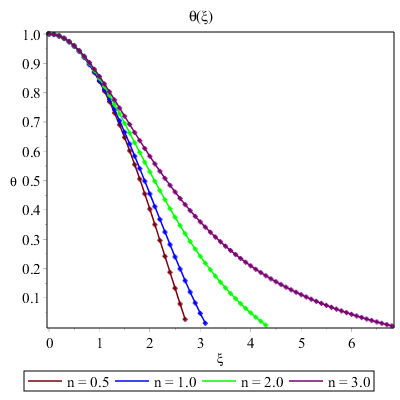
\includegraphics[scale=.7]{plots/laneEmden1.png}\\
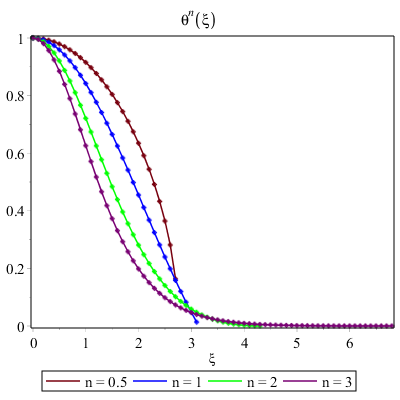
\includegraphics[scale=.7]{plots/laneEmden2.png}
\subsection*{Modelling Earth's Sun}
\begin{flalign*}
\rho_{unit} &= \frac{\Xi^3}{\hat M} \frac{M_\odot}{R_\odot} &&\\
& = \frac{6.897200^3}{ 25.361901} \frac{1.989 \times 10^{30} \textbf{kg}}{695700 \textbf{km}} && \\
 & = 3.6987 \times 10^{25} \frac{\textbf{kg}}{\textbf{km}}  = \rho_c && \\
\end{flalign*}

\begin{flalign*}
P_c &= \kappa \rho_c^{1+1/n} &&\\
\\
\kappa &= \frac{4\pi G \alpha^2}{n+1} \rho_c^{n-1/n} &&\\
\alpha &= \frac{R_\odot}{\Xi} = \frac{695700 \textbf{km}}{6.897} = 1.00869 \times 10^5 &&\\
\\
\kappa &= \frac{4 \pi (6.67 \times 10^{-14} \frac{\textbf{km}}{\textbf{s}^2})(1.00869 \times 10^5 \textbf{km})}{4} \rho_c^{2/3} &&\\
&= 2.113652 \times 10^-8 \rho_c^{2/3} &&\\
& = 2.346387 \times 10^9 &&\\
\\
P_c &= 2.346387 \times 10^9 \rho_c^{4/3} &&\\
&= 2.891560562*10^43 &&\\
\end{flalign*}
\section*{White Dwarfs}
\subsection*{$\pder[V]{s}$}
\begin{flalign*}
\frac{1}{s^2}\frac{d}{ds}\left (s^2 V G(\theta)\right ) & = - \theta &&\\
\frac{1}{s^2}\left [ 2sVG + s^2 \frac{d}{ds}(VG)\right ] & = - \theta &&\\
\frac{1}{s^2}\left [ 2sVG + s^2 \frac{dV}{ds}G + s^2V^2G'(\theta)\right ] & = - \theta &&\\
\frac{2VG}{s} +  \frac{dV}{ds}G + V^2G'  & = - \theta &&\\
 \frac{dV}{ds} &= \frac{2V}{s} - \frac{V^2G'}{G} - \frac{\theta}{G} &&\\
\end{flalign*}
\subsection*{Integrations for Selected Values of $\theta(0)$}
Full data outputs are available in the outputs directory.
\begin{tabular}{ | c c c |}

\multicolumn{3}{c}{ $\theta(0) = .05$ } \\
\hline
s & $\theta$ & $\hat M$\\
\hline
0 & .05 & 0 \\
5 & 0.003474 & 4.530548\\
10 & 0.000394 &8.354221 \\
15 & 0.000080& 10.060809 \\
16.8 & 0.000050& 10.421411\\
\hline
\end{tabular}\\
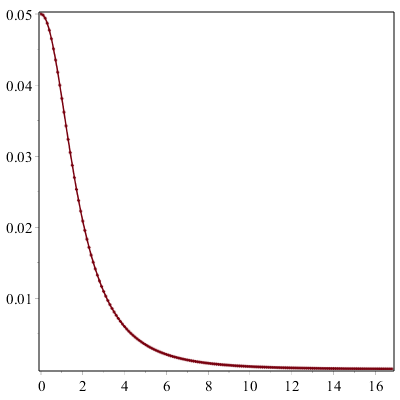
\includegraphics[scale=.5]{plots/wd1.png}\\
\begin{tabular}{ | c c c |}
\multicolumn{3}{c}{ $\theta(0) = .5$ } \\
\hline
s & $\theta$ & $\hat M$\\
\hline
0 & .5 & 0\\
3 &0.099983 & 23.313870 \\
6 & 0.009359& 44.747602\\
9 & 0.001821& 53.285835\\
12.1 & 0.000491 & 57.345664\\
\hline
\end{tabular}\\
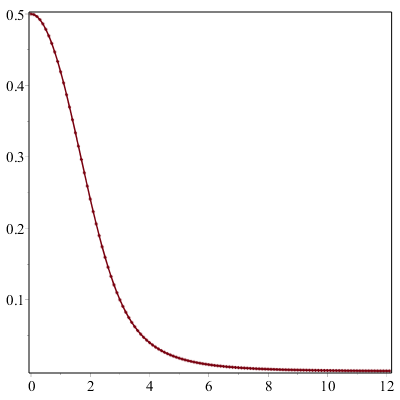
\includegraphics[scale=.5]{plots/wd2.png}\\
\begin{tabular}{ | c c c |}
\multicolumn{3}{c}{ $\theta(0) = 5$ } \\
\hline
s & $\theta$ & $\hat M$\\
\hline
0 & 5 & 0\\
2 &2.731982 &119.423255 \\
4 & 0.184593& 44.747602\\
6 & 0.021044& 365.125754\\
8.3 &0.004759 &379.679845\\
\hline
\end{tabular}\\
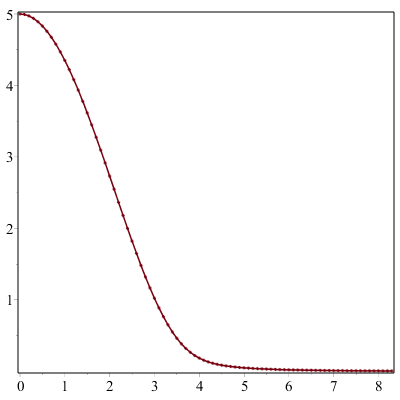
\includegraphics[scale=.5]{plots/wd3.png}\\
\begin{tabular}{ | c c c |}
\multicolumn{3}{c}{ $\theta(0) = 50$ } \\
\hline
s & $\theta$ & $\hat M$\\
\hline
0 & 50 & 0\\
1 &43.888692 &193.326200 \\
2 &28.244552&1217.559635\\
3 & 10.097859& 2635.815212\\
4.3 &0.045212 &3135.770481\\
\hline
\end{tabular}\\
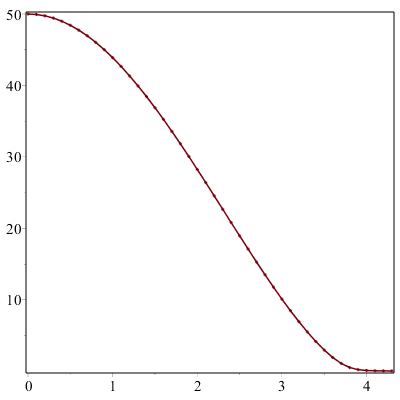
\includegraphics[scale=.5]{plots/wd4.png}\\
\begin{tabular}{ | c c c |}
\multicolumn{3}{c}{ $\theta(0) = 500$ } \\
\hline
s & $\theta$ & $\hat M$\\
\hline
0 & 500 & 0\\
1 &439.582357 &1940.891340 \\
2 &284.402935&12224.924810\\
3 & 100.083901& 26471.219489\\
3.7 &0.274937 &30576.933377\\
\hline
\end{tabular}\\
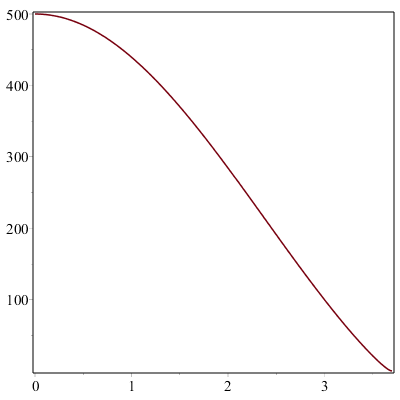
\includegraphics[scale=.5]{plots/wd5.png}\\
\begin{tabular}{ | c c c |}
\multicolumn{3}{c}{ $\theta(0) = 5000$ } \\
\hline
s & $\theta$ & $\hat M$\\
\hline
0 & 5000 & 0\\
1 &4397.550817&19413.417938\\
2 &2848.169588&122353.877586\\
3 & 997.874672& 264958.303355\\
3.64 &3.295236 &304300.467510\\
\hline
\end{tabular}\\
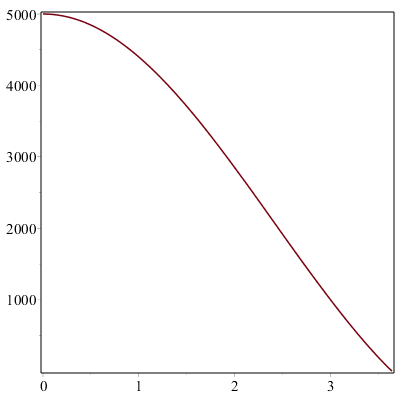
\includegraphics[scale=.5]{plots/wd6.png}\\
\begin{tabular}{ | c c c |}
\multicolumn{3}{c}{ $\theta(0) = 50000$ } \\
\hline
s & $\theta$ & $\hat M$\\
\hline
0 & 50000 & 0\\
1 &43979.215785&194143.848806\\
2 &28490.570788&1223763.244462\\
3 & 9971.996493& 2650101.145882\\
3.63 &22.034888 &3039898.580706\\
\hline
\end{tabular}\\
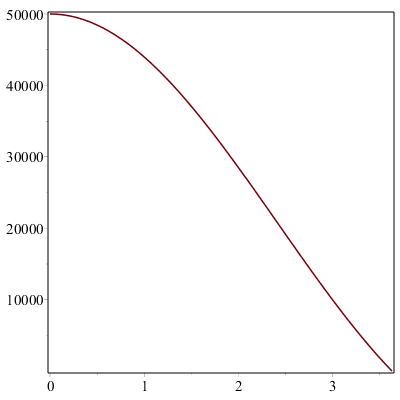
\includegraphics[scale=.5]{plots/wd7.png}\\
\begin{tabular}{ | c c c |}
\multicolumn{3}{c}{ $\theta(0) = 100000$ } \\
\hline
s & $\theta$ & $\hat M$\\
\hline
0 & 500000 & 0\\
1 &87959.184507&388289.661272\\
2 &56982.943351&2447572.068240\\
3 & 19942.606275& 5300307.090000\\
3.63 &16.402276 &6079172.237637\\
\hline
\end{tabular}\\
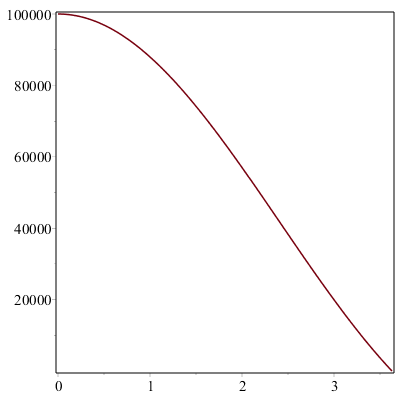
\includegraphics[scale=.5]{plots/wd8.png}\\



\subsection*{Mass-Radius Relation}
\textbf{Note:} The exact values here might be slightly off, due to $s_{max}$ being found with relatively low precision. This should not effect overall behavior.\\
\begin{tabular}{| c | c c |}
\hline
$\theta(0)$ & $\ln(M)$ & $\ln(R)$ \\
\hline
.05 & 74.07760638 & 21.68482052\\
.5 &75.78284118 & 21.35664709\\
5 &77.67307233 &20.97969715 \\
50 &79.78437413 & 20.32205666\\
500 & 82.06174514 & 20.17177446\\
5000 & 84.35951482& 20.15542532 \\
50000 &86.66107865 & 20.15267429 \\
500000 & 87.35412304& 20.15267429\\
\hline
\end{tabular}\\
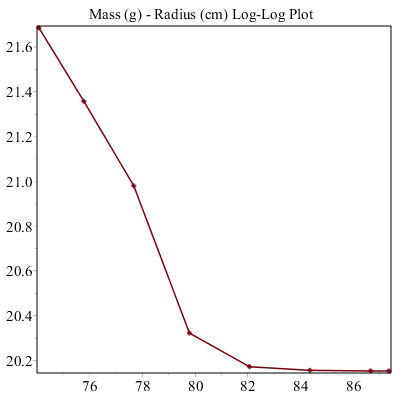
\includegraphics{plots/wdmassrad.png}
\end{document}
